\documentclass[10pt,twocolumn,letterpaper]{article}

\usepackage{cvpr}
\usepackage{times}
\usepackage{epsfig}
\usepackage{graphicx}
\usepackage{amsmath}
\usepackage{amssymb}

% Include other packages here, before hyperref.

% If you comment hyperref and then uncomment it, you should delete
% egpaper.aux before re-running latex.  (Or just hit 'q' on the first latex
% run, let it finish, and you should be clear).
\usepackage[breaklinks=true,bookmarks=false]{hyperref}

\cvprfinalcopy % *** Uncomment this line for the final submission

\def\cvprPaperID{****} % *** Enter the CVPR Paper ID here
\def\httilde{\mbox{\tt\raisebox{-.5ex}{\symbol{126}}}}

% Pages are numbered in submission mode, and unnumbered in camera-ready
%\ifcvprfinal\pagestyle{empty}\fi
\setcounter{page}{1}
\begin{document}

%%%%%%%%% TITLE
\title{Applying SlowFast Networks to Video Object Segmentation}

\author{Chantal Pellegrini\\
Technical University of Munich\\
{\tt\small chantal.pellegrini@tum.de}
% For a paper whose authors are all at the same institution,
% omit the following lines up until the closing ``}''.
% Additional authors and addresses can be added with ``\and'',
% just like the second author.
% To save space, use either the email address or home page, not both
\and
Ege Özsoy\\
	Technical University of Munich\\
	{\tt\small ege.oezsoy@tum.de}
}

\maketitle
%\thispagestyle{empty}

%%%%%%%%% ABSTRACT
\begin{abstract}
TALLE
\end{abstract}

% !TeX spellcheck = en_US
\section{Introduction}
The SlowFast architecture \cite{slow_fast}, which was successfully applied for video action classification, splits the workload between two branches, allowing it to use less memory. 
Our main goal is to apply SlowFast Networks \cite{slow_fast}  to Video Object Segmentation and to understand if this concept is beneficial for VOS; both in the unsupervised and semi-supervised settings. To this end, we build a SlowFast inspired VOS architecture, and evaluate different configurations of it.
% !TeX spellcheck = en_US
\section{Related Work}
The main work of consideration is the SlowFast Network \cite{slow_fast}, which has one fast and one slow pathway, allowing it to concentrate on different aspects of the video while keeping the performance high. The slow pathway is computationally much more expensive than the fast pathway and works with less frames. OSVOS \cite{osvos} focuses on the task of one-shot video object segmentation, where in test time, the network is fine-tuned on the first frame of the video, which has a manually annotated mask. This fine-tuning allows the network to adapt to the object in that video. Mask R-CNN \cite{mask_rcnn} is one of the best known architectures for image segmentation. They extend the popular Faster R-CNN architecture with a masking layer at the end.
% !TeX spellcheck = en_US
\section{Approach}
In the following we present the details of our approach.
\subsection{Dataset}
We used both of the DAVIS datasets \cite{davis_2016, davis_2017}. These datasets include videos with segmentation ground truths for every frame. We trained on DAVIS17, as it contains more video sequences, but evaluated on DAVIS16, which is a subset of DAVIS17, since there only exists one annotation per frame. %TODO do we need explanation?
\subsection{Network Design}
Our architecture mainly uses MaskRCNN, which we extended with a SlowFast module between the backbone and the head. An overview is shown in   Fig.~\ref{architecture}. The backbone is a ResNet50 Feature Pyramid Network, which was pretrained on Coco %TODO cite 
and fine-tuned on DAVIS17 \cite{davis_2017}.

The computed feature maps of several frames are fed into the SlowFast module, which can be seen in Fig.~\ref{slowfast}. It consists of two pathways, both with three 3D convolutions, followed by batch norm and for the first two layers a ReLu activation. After the first two layers the outputs of the fast pathway are fused into the slow pathway using another combination of Convolution, Batchnorm and ReLu.

The final outputs of the slow and the fast pathway are then concatenated and used as input for the Mask R-CNN head. Additionally the head also receives region proposals computed by a RPN, which works with the original image features computed by the backbone.

\begin{figure}
	\centering
	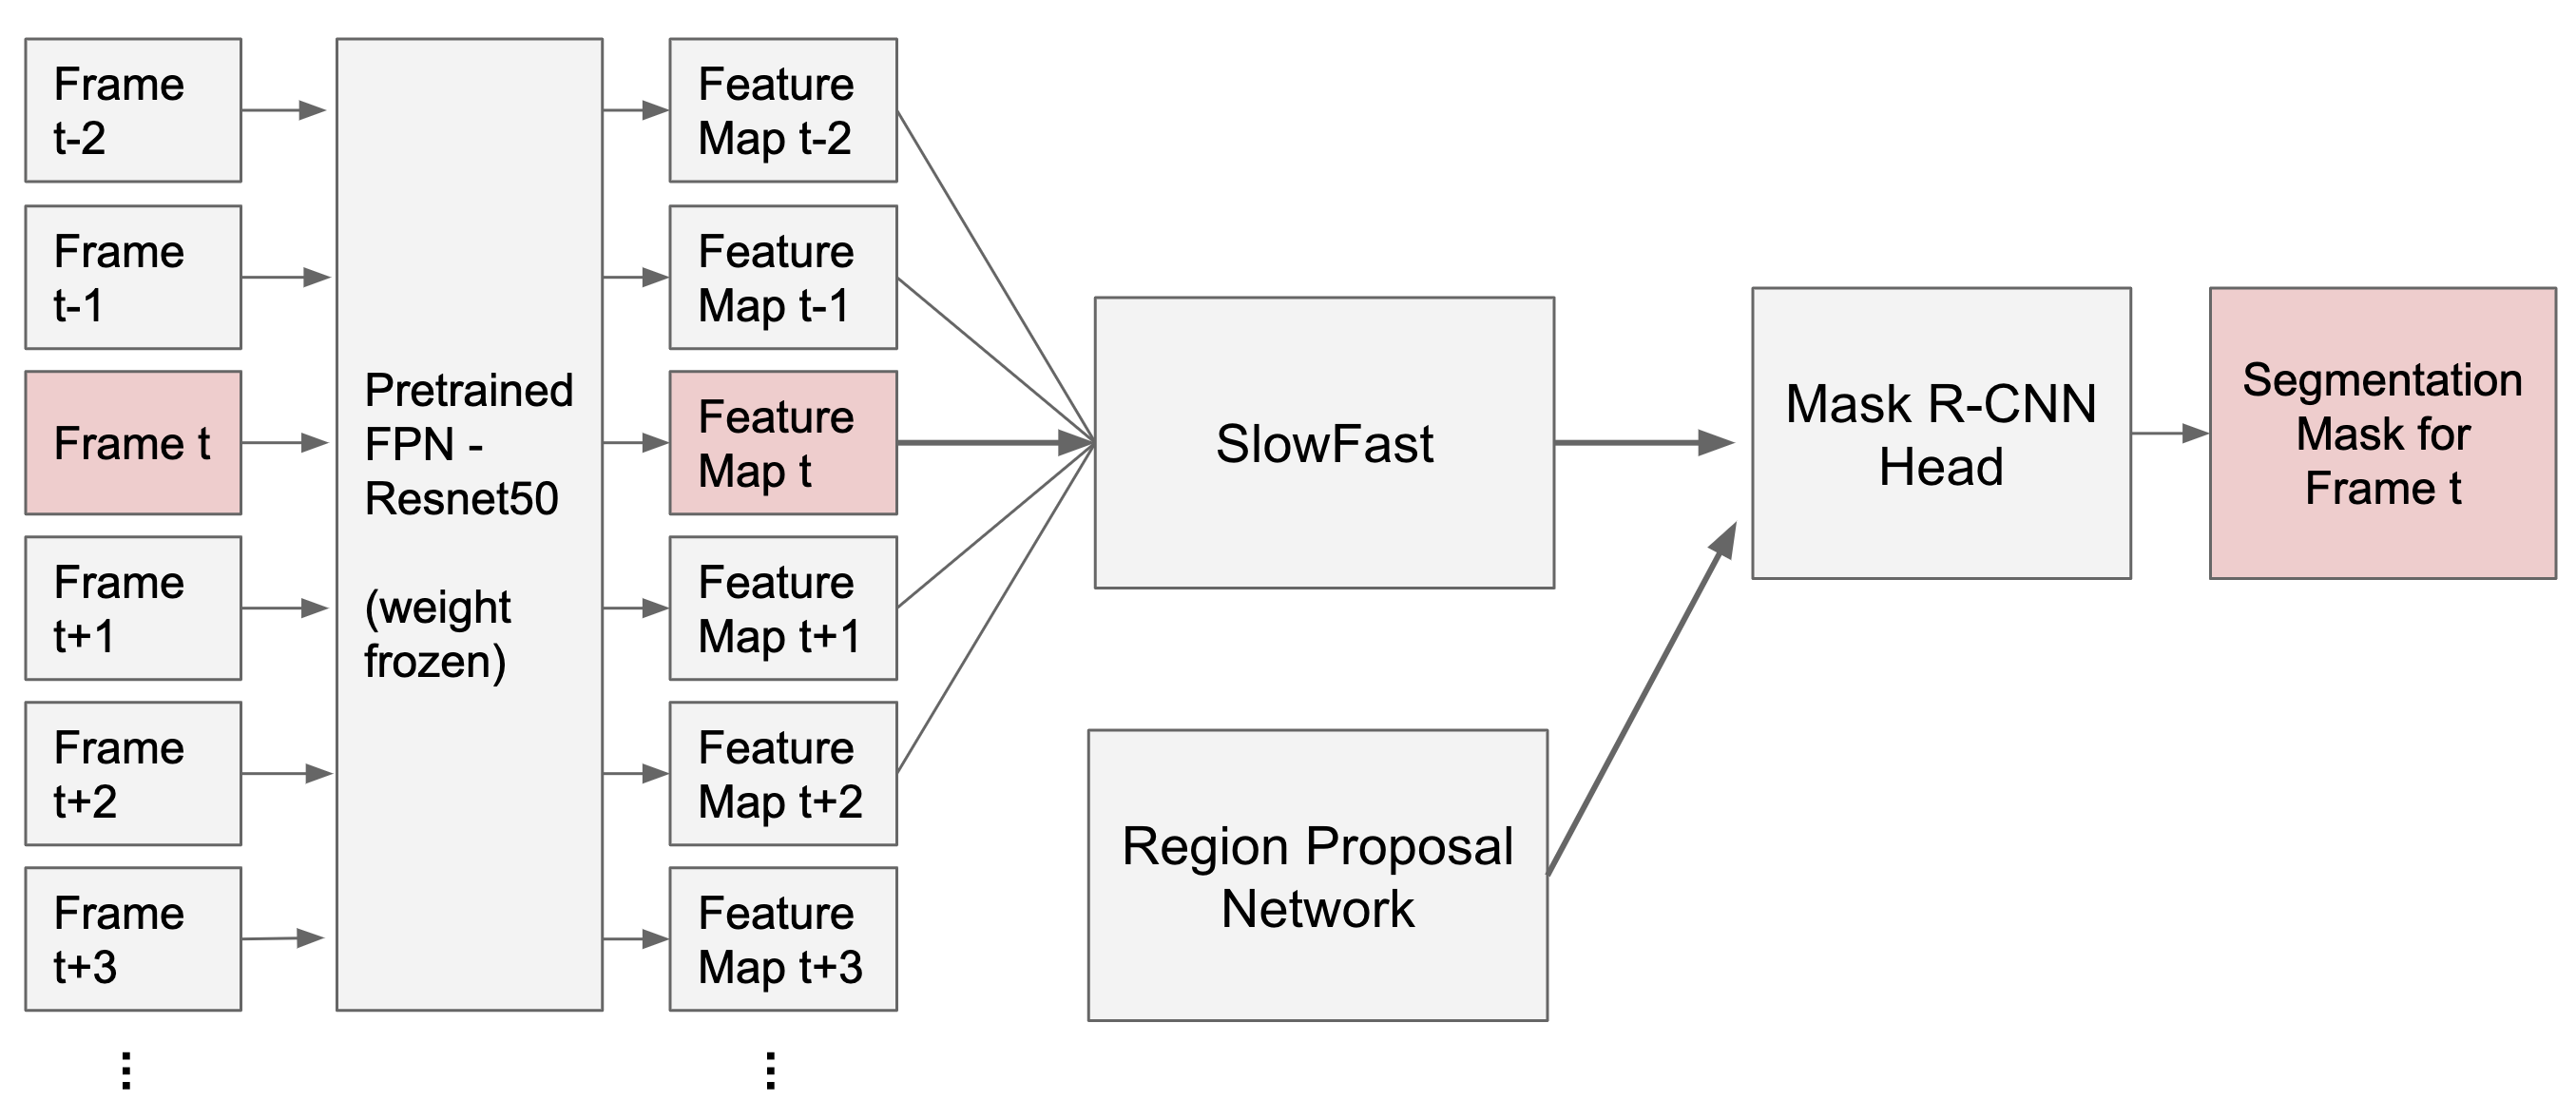
\includegraphics[width=\columnwidth]{figures/architecture.png}
	\caption{Architecture Overview.}
	\label{architecture}
\end{figure}

\begin{figure}
	\centering
	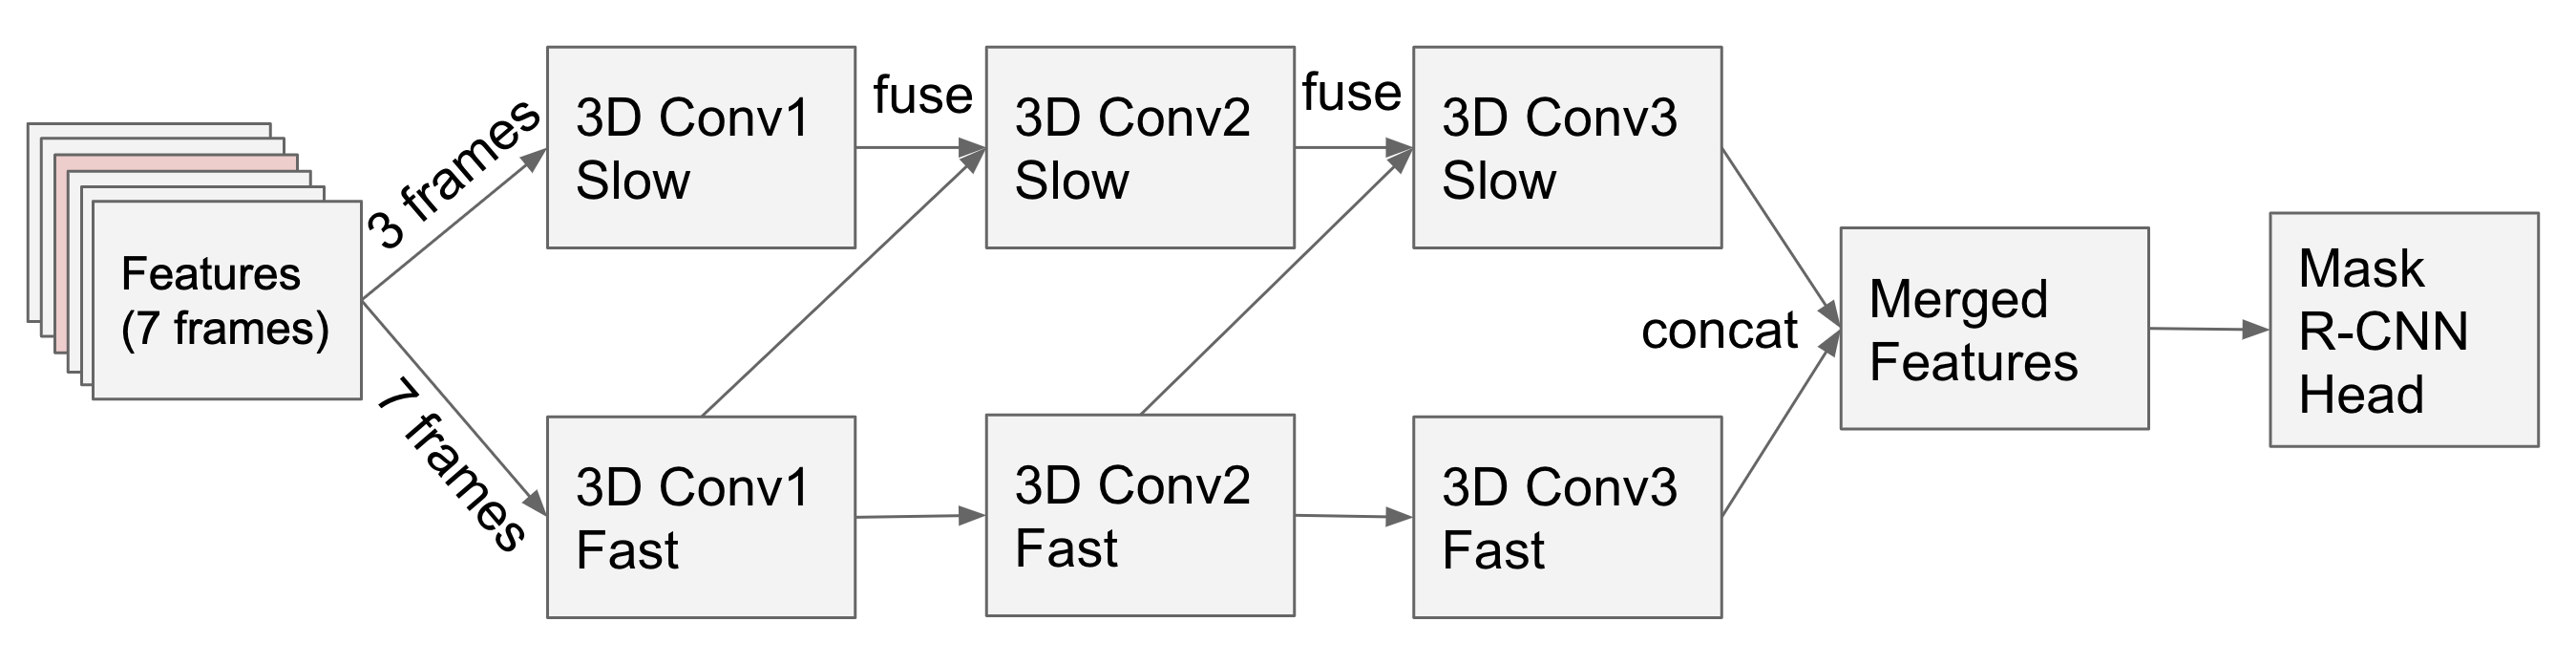
\includegraphics[width=\columnwidth]{figures/slowfast.png}
	\caption{Overview of SlowFast Layers.}
	\label{slowfast}
\end{figure}
\subsection{Training}
For the unsupervised case we are training for 20 epochs on the training data of DAVIS17 \cite{davis_2017}. We are using SGD with momentum as optimizer and our learning rate is set to 0.001.

The semi-supervised training starts with a parent model trained on the task of unsupervised VOS and finetunes this model on specific sequences, resulting in one model per sequence. We are using different augmentations, including Random Horizontal Flip, Rotation of up to 30 degrees, and Scaling of the image. We experimented with different scaling strengths and learning rates, that are described in the experiment section.
% !TeX spellcheck = en_US
\section{Experiments}
We conducted several experiments for both hyper-parameter tuning and the evaluation of different configurations.
The qualitative results can be found here \url{https://www.youtube.com/playlist?list=PLog3nOPCjKBnjhuHMIXu4ISE4Z4f2jm39}
%TODO qualitative link

\subsection{Hyperparameter Search}
As our resources were limited, we relied on previous works for some decisions such as which optimizer to use. Nonetheless, for the unsupervised case, we experimented with 3 different learning rates and also freezing the backbone or not. In the end we settled on 0.001 as lr and freezing the backbone, as training it did not provide much improvement but came at a big cost of speed. For the semi-supervised case we ran 36 experiments for every pathway configuration, which tested different settings for data augmentation, learning rate and freezing different parts of the network. Following the results we freeze only the SlowFast part of the network and use a random scale of 0.25 or 0.4 (only for 1-1) and learning rate of 0.001.

\subsection{Pathway Configurations}
The main goal of the pathway configurations is to show the benefit of more temporal context and the SlowFast concept. We denote our configurations as m-n, where m/n refers to the number of frames given to the slow/fast pathway.
We create a baseline configuration, 1-1, which does not use any temporal context and two additional architectures 3-3 and 7-7 which progressively use more temporal context. These three configurations are not using a SlowFast inspired architecture, as both of the pathways have the same size. In addition to these three, we test 1-7 and 3-7, both utilizing the concept of SlowFast.

\subsection{Results}
Table~\ref{unsupervised_results} and \ref{semi_supervised_results} show the results for the unsupervised, respectively semi-supervised experiments. As evaluation metric we use J\&F Mean, like described in the DAVIS16\cite{davis_2016}.
\begin{table}[]
	\centering
	\begin{tabular}{|c|c|c|c|}
		\cline{1-4}
		Configuration & J \& F Mean & Param. Count & Eval. Time \\ \cline{1-4}
		1-1  & 0.645  & 45,421,851 & 477 sec\\ \cline{1-4}
		3-3    & 0.679 & 46,398,747 & 544 sec\\ \cline{1-4}
		7-7    & 0.673 & 48,407,835 & 853 sec\\ \cline{1-4}
		1-7    & 0.655  & 45,618,459 & 528 sec\\ \cline{1-4}
		3-7    & 0.676  & 46,570,779 & 584 sec\\ \cline{1-4}
	\end{tabular}
	\caption{Unsupervised VOS results on DAVIS16 validation set. The Evaluation Time refers to computation of masks for all validation sequences.}
	\label{unsupervised_results}
\end{table}

\begin{table}[]
	\centering
	\begin{tabular}{|c|c|}
		\cline{1-2}
		Configuration & J \& F Mean\\ \cline{1-2}
		1-1  & 0.747  \\ \cline{1-2}
		3-3    & 0.747 \\ \cline{1-2}
		7-7    & 0.755 \\ \cline{1-2}
		1-7    & 0.741  \\ \cline{1-2}
		3-7    & 0.758  \\ \cline{1-2}
	\end{tabular}
	\caption{Semi-supervised VOS results on DAVIS16 validation set.}
	\label{semi_supervised_results}
\end{table}

% !TeX spellcheck = en_US
\section{Evaluation}
Our first observation is that in our case temporal context improves the unsupervised segmentation results, but only up to three frames, as can be seen by comparing the results of 1-1, 3-3 and 7-7. As SlowFast networks are mainly designed to see a lot of temporal context in the fast pathway and this does not seem to be beneficial here, the potential benefit is small. When we compare 1-1 to 1-7 and 3-3 to 3-7 we only see an improvement through a larger fast pathway size for a slow pathway size of one.

In the semi-supervised experiments we only see little temporal benefit between 3-3 and 7-7 and none between 1-1 and 3-3. We also see a small improvement between 3-3 and 3-7 but a small regression from 1-1 to 1-7. Overall the small differences indicate neither temporal context nor SlowFast have significant influence on the OSVOS results.

Performance wise the parameter count increases with bigger pathway sizes, but the evaluation time increases significantly. The slow pathway has significantly more influence on both, as can be seen by comparing 3-3, 3-7 and 7-7.

Overall the benefit of SlowFast for our tasks appears to be limited. 
% !TeX spellcheck = en_US
\section{Conclusion}
In this project our goal was to implement a SlowFast inspired architecture for video object segmentation, and thereby investigate the potential benefit of SlowFast Networks for VOS. The takeaway from our results is that there was no substantial benefit observed from applying SlowFast, especially because the benefit of having more and more temporal context vanished quickly. In the cases where a temporal benefit was observed, SlowFast improved the results with little performance overhead.

{\small
\bibliographystyle{ieee_fullname}
\bibliography{egbib}
}

\end{document}
